%%%%%%%%%%%%%%%%%%%%%%%%%%%%%%%%%%%%%%%%%%%%%%%%%%%%%%%%%%%%%%%%%%%%
%% I, the copyright holder of this work, release this work into the
%% public domain. This applies worldwide. In some countries this may
%% not be legally possible; if so: I grant anyone the right to use
%% this work for any purpose, without any conditions, unless such
%% conditions are required by law.
%%%%%%%%%%%%%%%%%%%%%%%%%%%%%%%%%%%%%%%%%%%%%%%%%%%%%%%%%%%%%%%%%%%%

\documentclass{beamer}
\usepackage{graphicx}
\usepackage{multicol}
\usetheme[faculty=fi]{fibeamer}
\usepackage[utf8]{inputenc}
\usepackage[
  main=english, %% By using `czech` or `slovak` as the main locale
                %% instead of `english`, you can typeset the
                %% presentation in either Czech or Slovak,
                %% respectively.
  czech, slovak %% The additional keys allow foreign texts to be
]{babel}        %% typeset as follows:
%%
%%   \begin{otherlanguage}{czech}   ... \end{otherlanguage}
%%   \begin{otherlanguage}{slovak}  ... \end{otherlanguage}
%%
%% These macros specify information about the presentation


 
\title{\hspace{45mm} Rayos X} %% that will be typeset on the
\subtitle{\textbf{Introducci\'on a f\'isica moderna}} %% title page.
\author{Integrantes: \hspace{65mm}Profesor:\\Miguel Ernesto Medina Le\'on \hspace{40mm} El Kiks \\Llanet Ramos Valenzuela\\Luis Aaron Cer\'on Ram\'irez}
%% These additional packages are used within the document:
\usepackage{ragged2e}  % `\justifying` text
\usepackage{booktabs}  % Tables
\usepackage{tabularx}
\usepackage{tikz}      % Diagrams
\usetikzlibrary{calc, shapes, backgrounds}
\usepackage{amsmath, amssymb}
\usepackage{url}       % `\url`s
\usepackage{listings}  % Code listings
\frenchspacing
\begin{document}
  \frame{\maketitle}

  \AtBeginSection[]{% Imprime el índice por cada sección
    \begin{frame}<beamer>
      \frametitle{\'Indice}
      \tableofcontents[currentsection]
    \end{frame}}

  \begin{darkframes} %Inician las diapositivas oscuras.
    \section{Historia} %Título que aparece en el índice
    \begin{frame}{Historia} %Título que aparece en la diapositiva
      \framesubtitle{Un poco de contexto} %Subtítulo
     \begin{multicols}{2}
     \begin{figure}
         \centering
         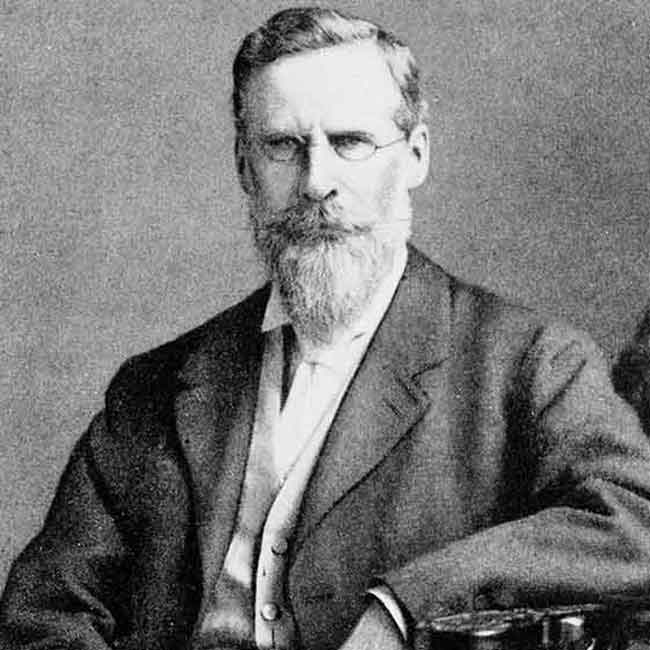
\includegraphics[width = 0.85 \linewidth]{resources/1f.jpg}
         \caption{William Crookes (Londres, Inglaterra. 17 de Junio de 1832 - Londres, Inglaterra. 4 de Abril de 1919).}
         \label{fig:my_label}
     \end{figure}
     
     \newpage
     \begin{figure}
         \centering
         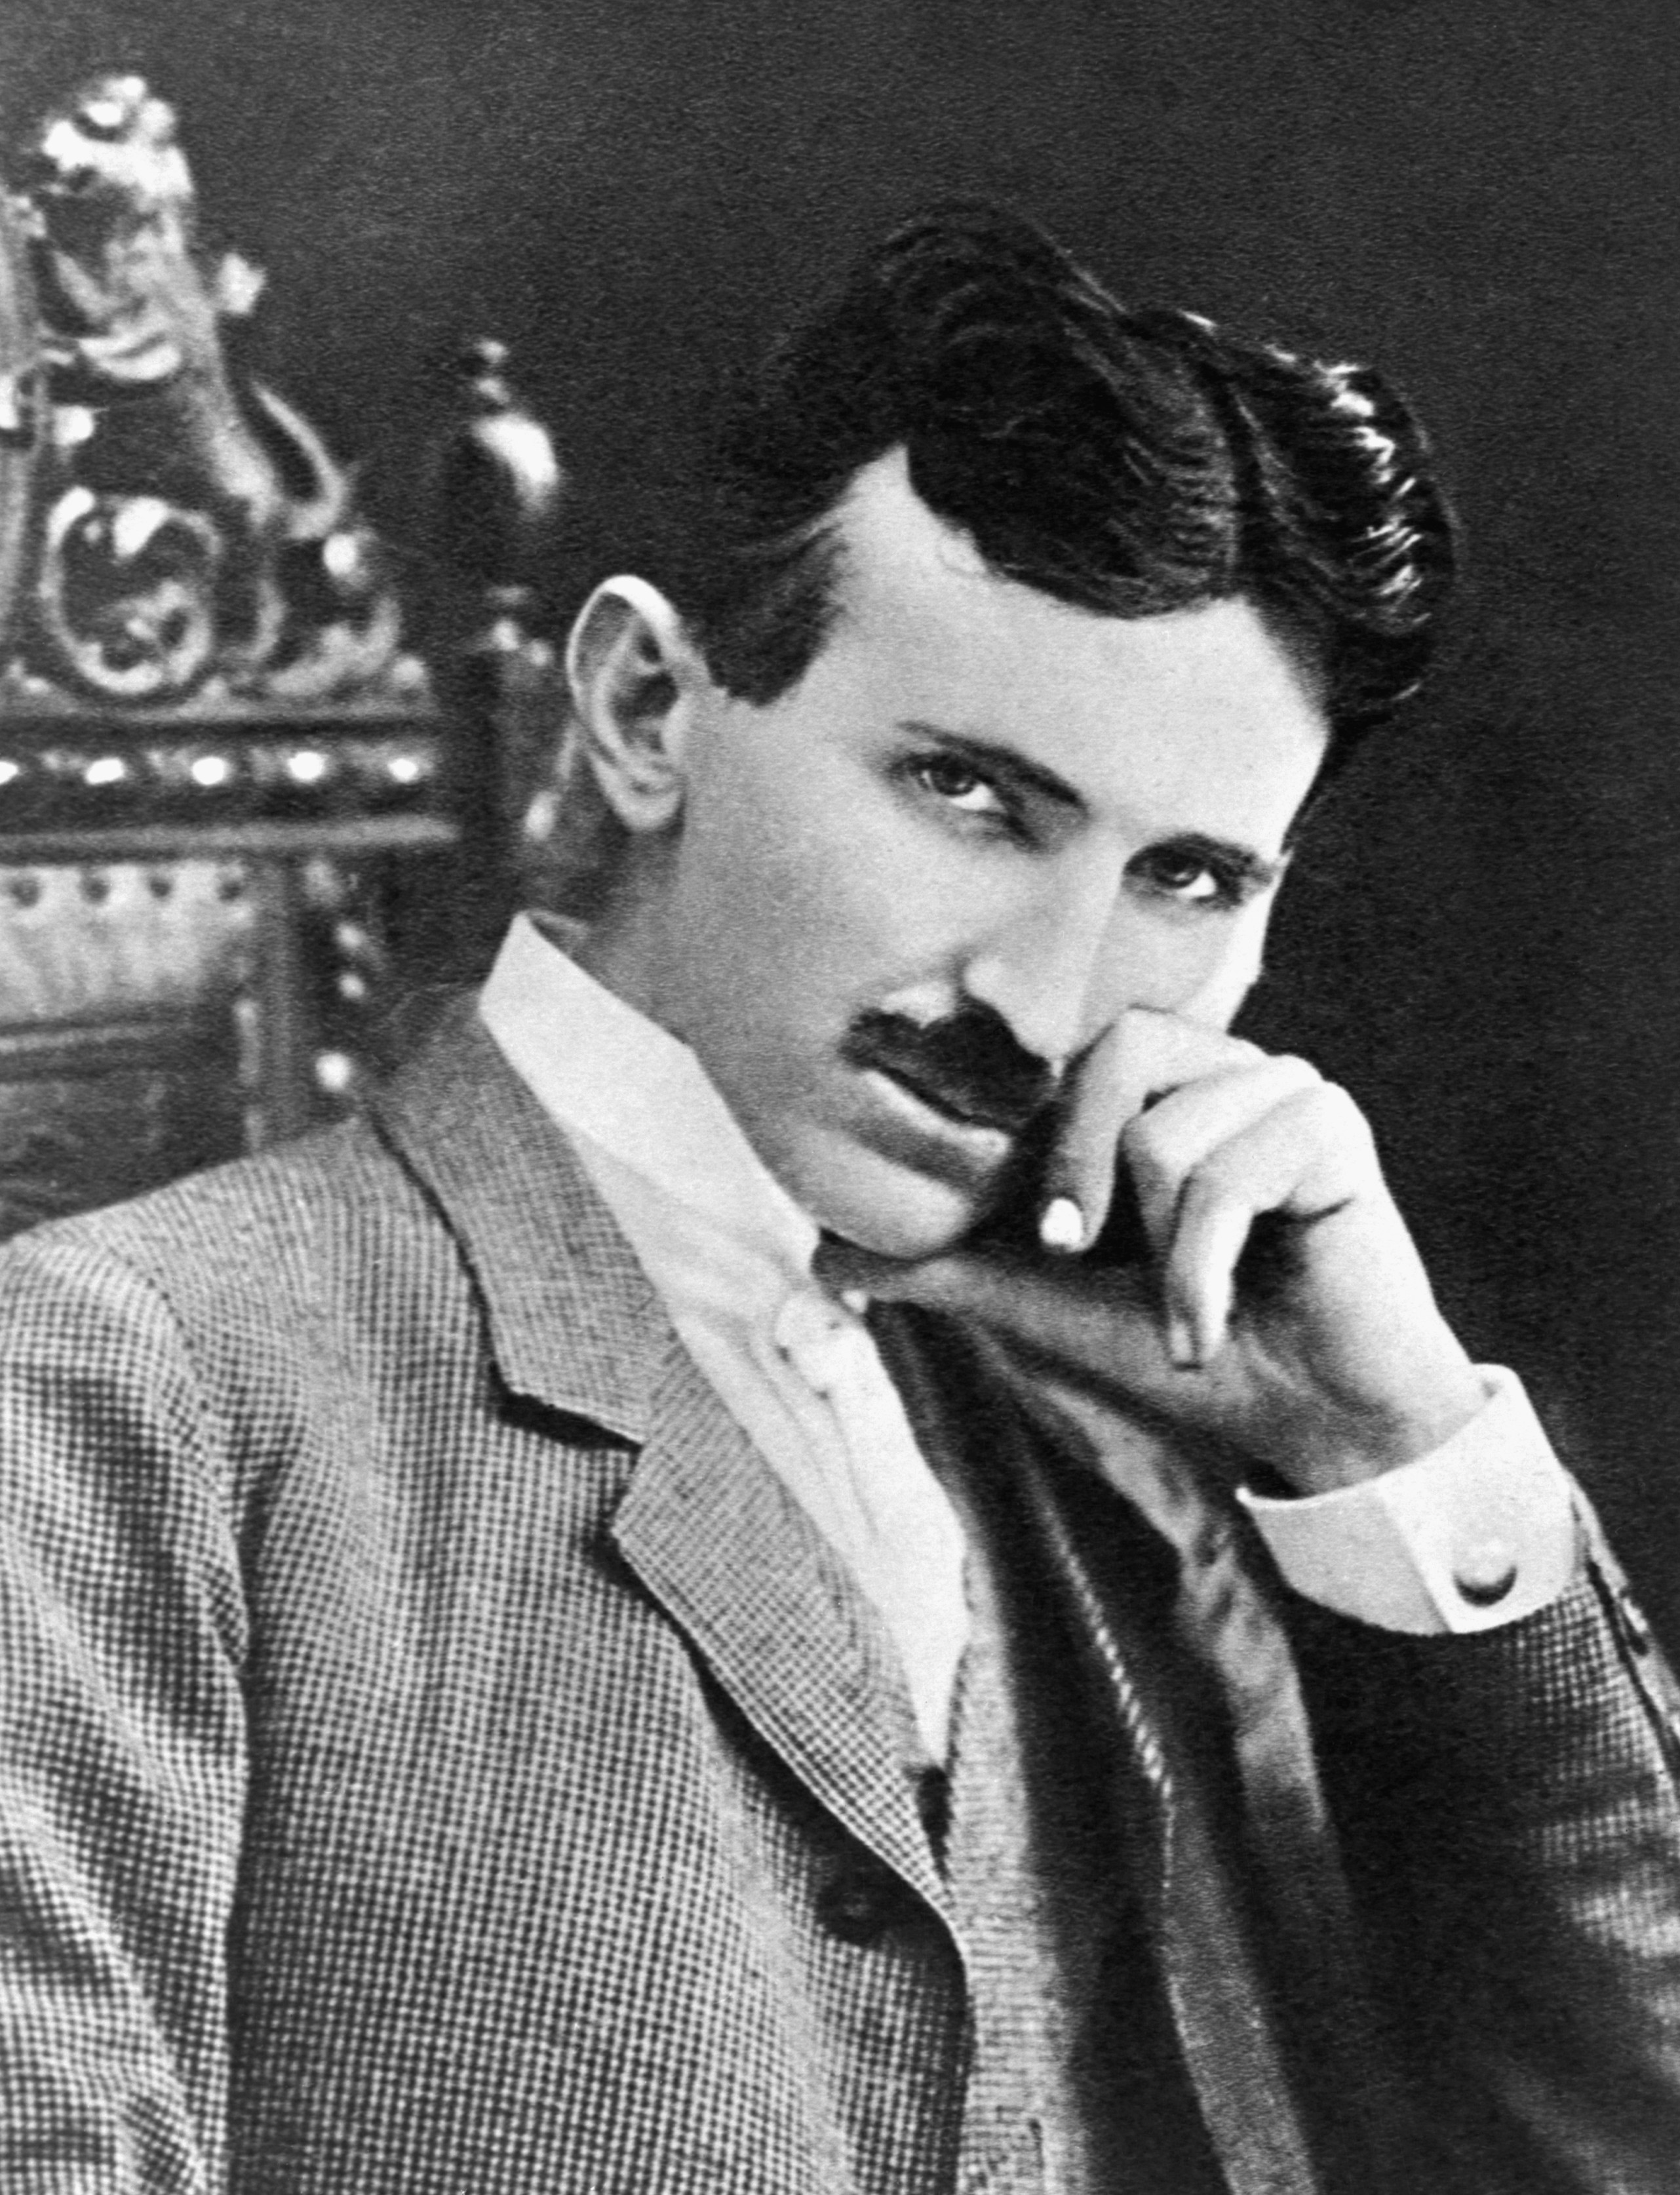
\includegraphics[width = 0.7 \linewidth]{resources/2f.jpg}
         \caption{Nikola Tesla (Smiljan, Croacia. 10 de Julio de 1856 - Nueva York, EUA. 7 de Enero de 1943).}
         \label{fig:my_label}
     \end{figure}
     
      
    \end{multicols}
    \end{frame}


    \begin{frame} %Título que aparece en la diapositiva
      \framesubtitle{El principal aportador} %Subtítulo
        
        \begin{multicols}{2}
     \begin{figure}
         \centering
         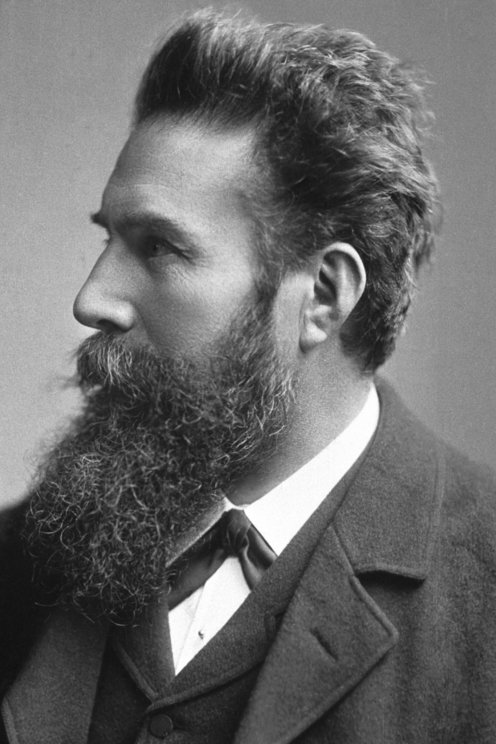
\includegraphics[width = 0.85 \linewidth]{resources/3f.jpg}
         \caption{Wilhelm Conrad Röntgen (Remscheid, Alemania. 27 de Marzo de 1845 - Munich, Alemania. 10 de Febrero de 1923).}
         \label{fig:my_label}
     \end{figure}
     
     \newpage
     \begin{figure}
         \centering
         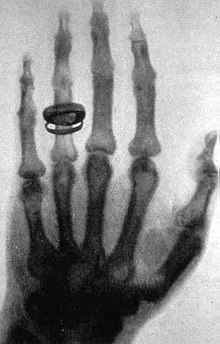
\includegraphics[width = 0.85 \linewidth]{resources/4f.jpg}
         \caption{Anna Bertha Ludwig Röntgen. Foto tomada el 22 de Diciembre de 1895.}
         \label{fig:my_label}
     \end{figure}
  
      \end{multicols}
    \end{frame}

    \section{Experimento} %Título que aparece en el índice
    \begin{frame}{El experimento de Röntgen} %Título que aparece en la diapositiva
      \framesubtitle{Detectando los rayos inc\'ognita} %Subtítulo
     
     \begin{multicols}{2}
     \begin{figure}
         \centering
         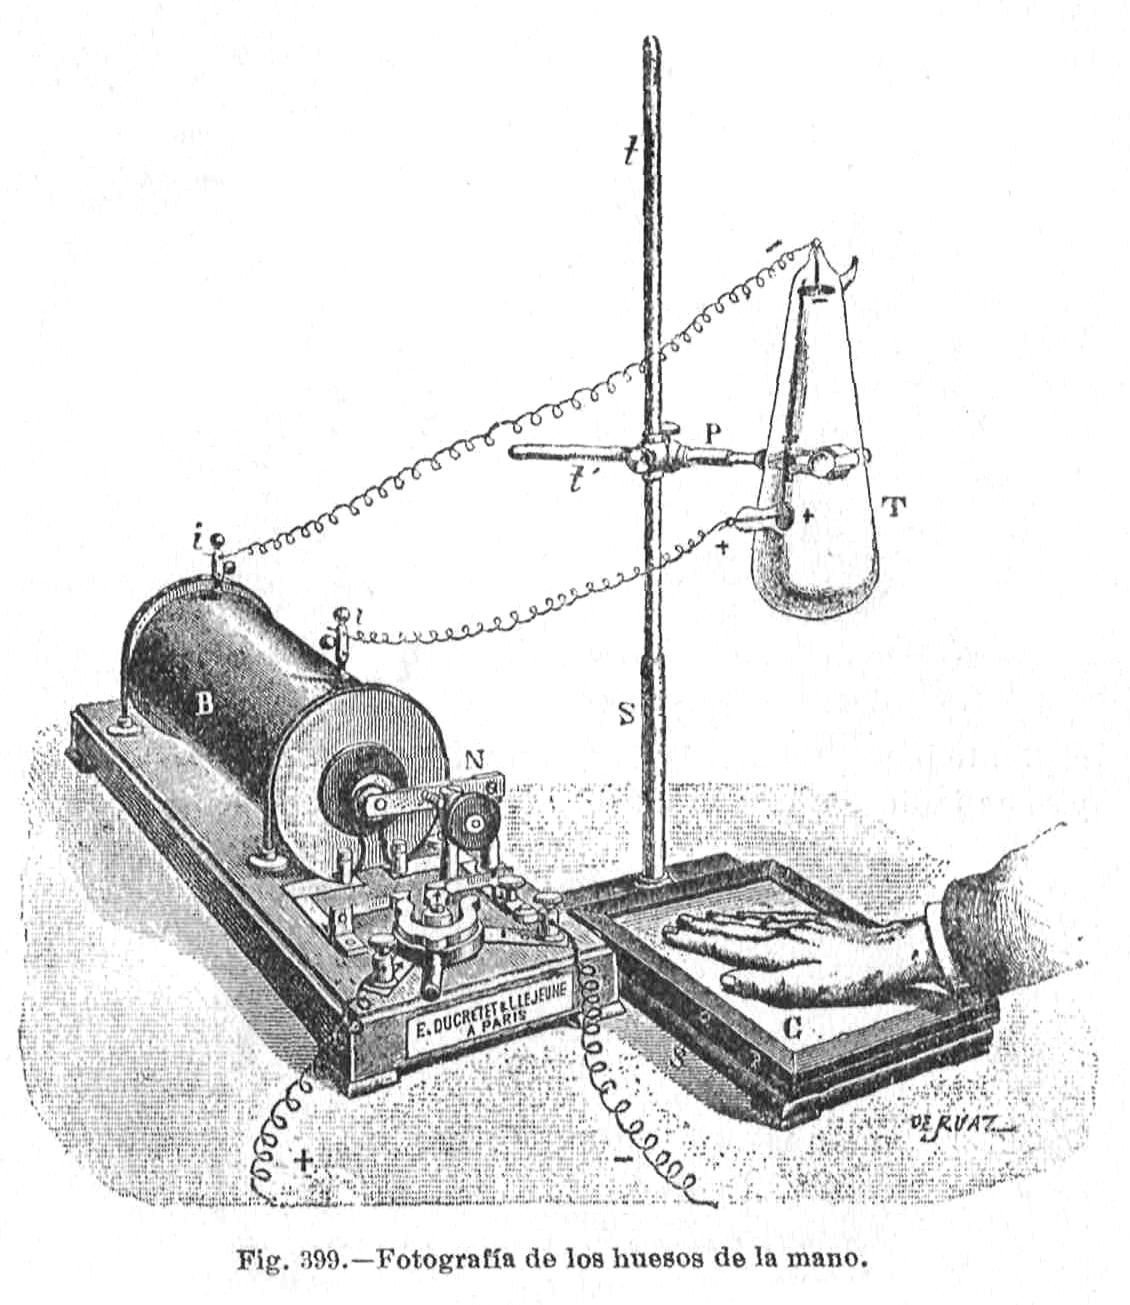
\includegraphics[width = 0.75 \linewidth]{resources/20f.jpg}
         \caption{"Elementos de Física", Eduardo Lozano y Ponce de León, Establecimiento Tipográfico de Jaime Ratés, Madrid 1907}
         \label{fig:my_label}
     \end{figure}
     
     \newpage
     \begin{figure}
         \centering
         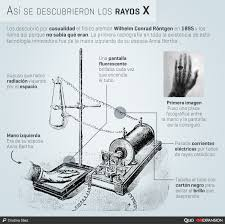
\includegraphics[width = 1 \linewidth]{resources/21f.jpeg}
         \caption{Representaci\'on y dibujo del antiguo experimento.}
         \label{fig:my_label}
     \end{figure}
     
     
     \end{multicols}

    \end{frame}
    
    
    \section{Antecedentes te\'oricos}
    \begin{frame}{La luz}
    \framesubtitle{El misterio corpuscular}
    \begin{figure}
        \centering
        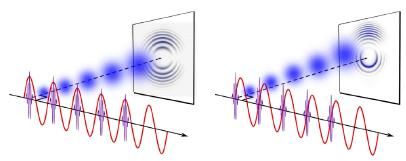
\includegraphics[width = 0.8 \linewidth]{resources/22.jpg}
    \end{figure}
    
    En la \'epoca de Isaac Newton, la mayor\'ia de cient\'ificos pensaban que la luz consist\'ia en corrientes de part\'iculas (llamadas corp\'usculos) emitidas por las fuentes luminosas. Galileo y otros intentaron medir la rapidez de la luz. 
    Alrededor de 1665, comenzaron a descubrirse evidencias de las propiedades ondulatorias de la luz.
    
    \end{frame}
    
    
    \begin{frame}{El espectro electromagn\'etico}
    \framesubtitle{Al descubierto}
    
    \begin{figure}
        \centering
        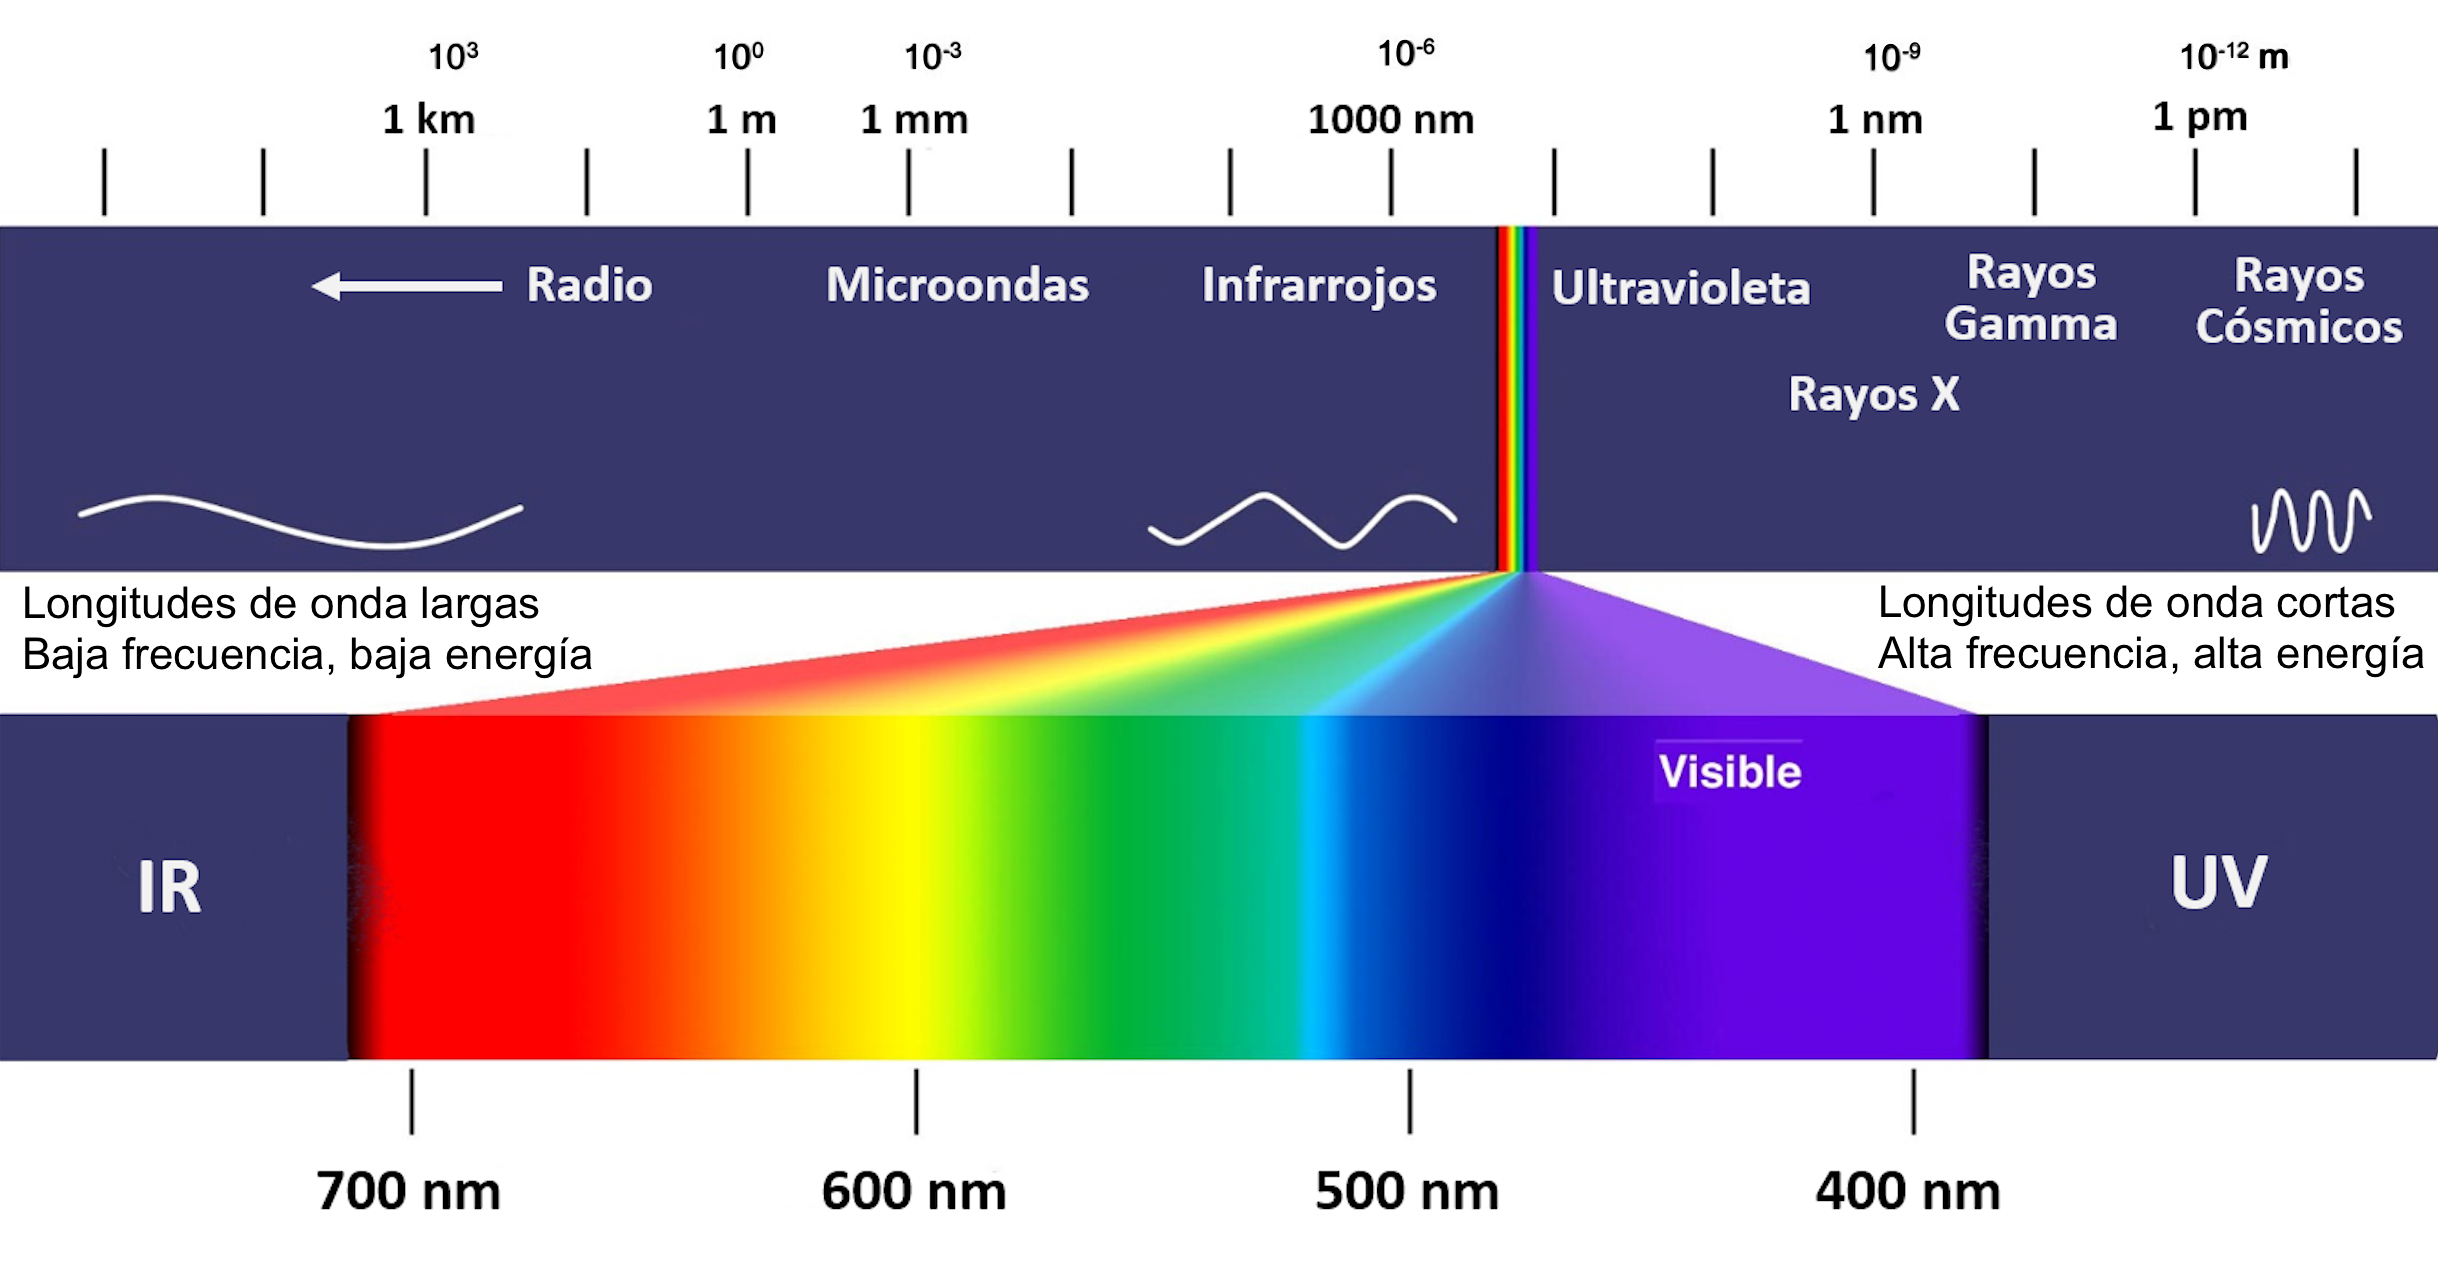
\includegraphics[width = 0.65 \linewidth]{resources/23.png}
    \end{figure}
    
    El espectro electromagn\'etico es un conjunto de ondas que van desde las que poseen una mayor longitud como las ondas de radio, hasta las que tienen menor longitud como los rayos $\gamma$. \'Estas se pueden clasificar y ordenar de acuerdo a sus diferentes longitudes de onda y frecuencias.
    
    \end{frame}
    
    \section{Rayos X} %Título que aparece en el índice
    \begin{frame}{Definici\'on} %Título que aparece en la diapositiva
      \framesubtitle{Entendiendo algunos conceptos} %Subtítulo
      \begin{itemize}
          \item \textbf{Radiaci\'on} (del lat\'in radiatio, $\tilde{o}$nis "resplandor")
          \begin{itemize}
          \item Acci\'on y efecto de irradiar.
          \item Energ\'ia ondulatoria o part\'iculas materiales que se propagan a trav\'es del espacio.
          \item Forma de propagarse de la energ\'ia o las part\'iculas.
          \end{itemize}
          Esta energ\'ia puede propagarse por medio de \textit{part\'iculas subat\'omicas} o por medio de \textit{ondas electromagn\'eticas}. 
      \end{itemize}
      

    \end{frame}
    
    \begin{frame}{Definici\'on} %Título que aparece en la diapositiva
      \begin{itemize}
          \item \textbf{Radiactividad}
          \begin{itemize}
          \item Propiedad de ciertos cuerpos cuyos \'atomos, al desintegrarse espont\'aneamente, emiten radiaciones.
          \end{itemize}
          \begin{tikzpicture}[overlay,remember picture] %Comando para fotos que forman parte de la diapositiva
        \node[anchor=south east,xshift=-105pt,yshift=70pt] %Comando para mover la foto
          at (current page.south east) {
            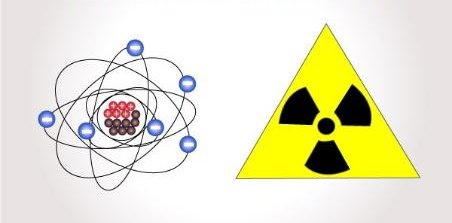
\includegraphics[width=45mm]{resources/11f.jpg} %Aquí se adjunta la foto como propiedad de la carpeta Resources
          };
      \end{tikzpicture}%
      \vfill
      \vfill
      \vfill
      Existen tres tipos de radiaci\'on.
      \end{itemize}
      

    \end{frame}
    
    
    \begin{frame}{Radiaci\'on $\alpha$} %Título que aparece en la diapositiva
      \begin{tikzpicture}[overlay,remember picture] %Comando para fotos que forman parte de la diapositiva
        \node[anchor=south east,xshift=-15pt,yshift=75pt] %Comando para mover la foto
          at (current page.south east) {
            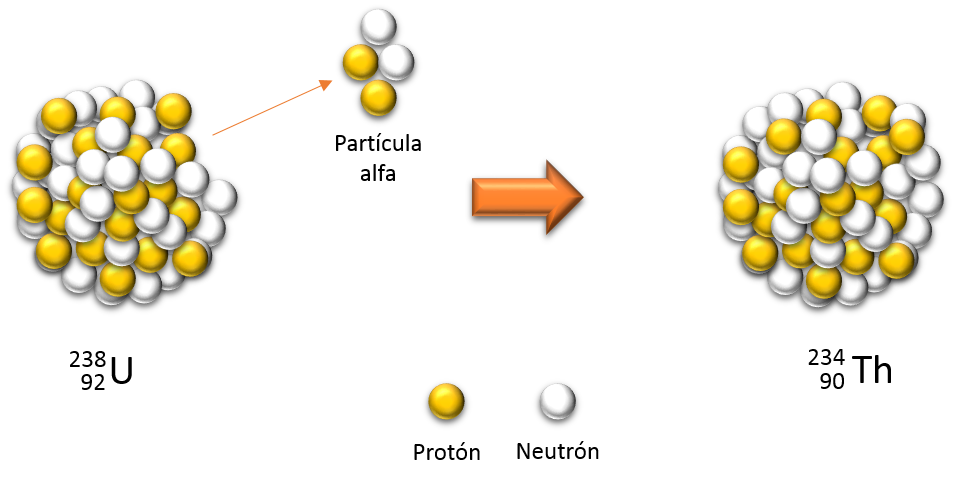
\includegraphics[width=45mm]{resources/10f.png} %Aquí se adjunta la foto como propiedad de la carpeta Resources
          };
      \end{tikzpicture}%
        Son part\'iculas constituidas por dos protones y dos neutrones, cargadas positivamente y emitidas por ciertas sustancias radiactivas.
        \framesubsubtitle{\textbf{Caracter\'isticas}}
        \begin{itemize}
            \item Son de baja velocidad.
            \item Lentas y pesadas.
            \item Alta transferencia de energ\'ia lineal.
            \item Produce ionizaci\'on.
            \item Puede ser detenida por una hoja de papel.
        \end{itemize}
    \end{frame}
    
    
    \begin{frame}{Radiaci\'on $\beta$} %Título que aparece en la diapositiva
      \begin{tikzpicture}[overlay,remember picture] %Comando para fotos que forman parte de la diapositiva
        \node[anchor=south east,xshift=-20pt,yshift=30pt] %Comando para mover la foto
          at (current page.south east) {
            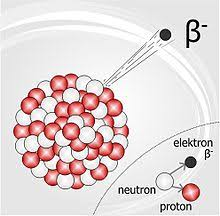
\includegraphics[width=30mm]{resources/12f.jpeg} %Aquí se adjunta la foto como propiedad de la carpeta Resources
          };
      \end{tikzpicture}%
        Son, tanto electrones como positrones, expulsadas a altas velocidades del n\'ucleo y emitidas por sustancias radiactivas.
        \framsubsubtitle{\bf Caracter\'isticas}
        \begin{itemize}
            \item De mayor rango y velodidad que las alfa, pero de menor masa.
            \item Menor transferencia de energ\'ia lineal.
            \item Produce ionizaci\'on, pero menor que las alfa.
            \item Pueden ser detenidas por el aluminio.
        \end{itemize}
    \end{frame}
    
    \begin{frame}{Radiaci\'on $\gamma$} %Título que aparece en la diapositiva
      \begin{tikzpicture}[overlay,remember picture] %Comando para fotos que forman parte de la diapositiva
        \node[anchor=south east,xshift=-105pt,yshift=90pt] %Comando para mover la foto
          at (current page.south east) {
            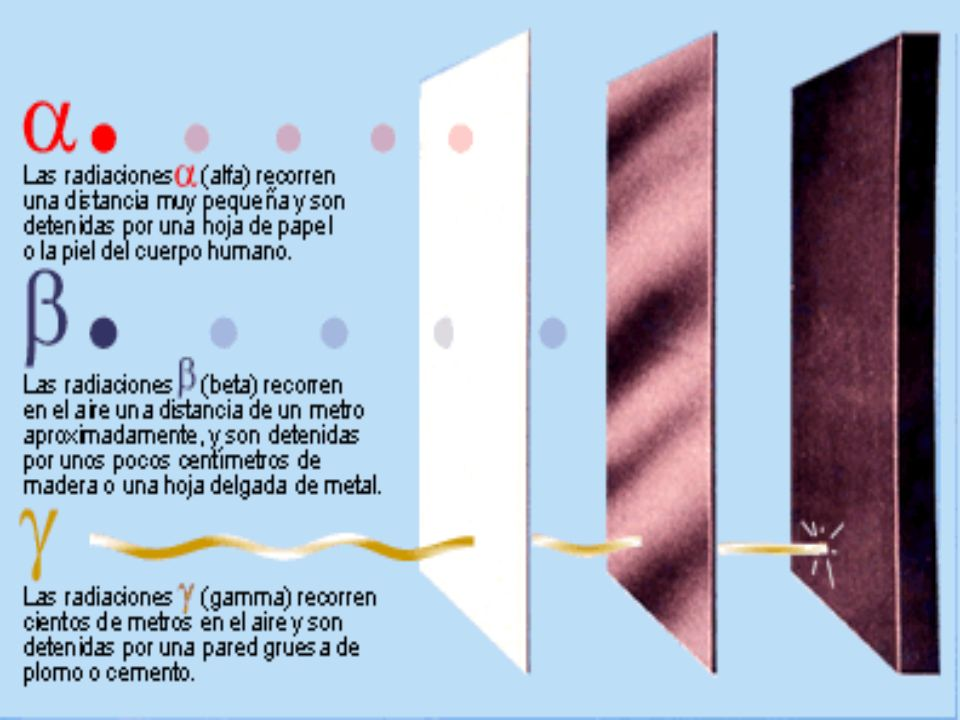
\includegraphics[width=60mm]{resources/13f.jpg} %Aquí se adjunta la foto como propiedad de la carpeta Resources
          };
      \end{tikzpicture}%
      \vfill
        \vfill
        \vfill
        \vfill
        \RaggedDown{Radiaci\'on electromagn\'etica de gran poder de penetraci\'on, la cual es emitida por el n\'ucleo de una sustancia radiactiva o por aniquilaci\'on de un par electr\'on-positr\'on.}
    \end{frame}
    
     \begin{frame}{\hspace{45mm}Rayos X}
     %\framesubtitle{?`Qu\'e son?}%Título que aparece en la diapositiva
      \begin{tikzpicture}[overlay,remember picture] %Comando para fotos que forman parte de la diapositiva
        \node[anchor=south east,xshift=-70pt,yshift=94pt] %Comando para mover la foto
          at (current page.south east) {
            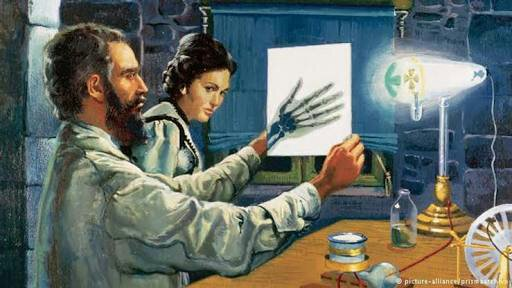
\includegraphics[width=80mm]{resources/26f.jpg} %Aquí se adjunta la foto como propiedad de la carpeta Resources
          };
      \end{tikzpicture}%
      \vfill
        \vfill
        \vfill
        \vfill
        \RaggedDown{Los rayos X son radiaciones electromagn\'eticas cuya longitud de onda es del orden de 10 a 0.01 nm, correspondiendo a frecuencias en el rango de 30 a 30000 PHz (de 50 a 50000 veces la frecuencia de la luz visible). }
    \end{frame}
    
    \begin{frame}{Caracter\'isticas de los rayos X}
    \begin{itemize}
        \item Penetran cuerpos opacos.
        \item Sensibilizan placas radiogr\'aficas.
        \item Producen fluorescencia.
        \item Producen efectos biol\'ogicos en los seres vivos.
        \item Son divergentes.
        \item Viajan en l\'inea recta.
        \item Invisibles; no se reflejan ni se refractan.
        \item Sin masa ni carga. 
    \end{itemize}
    
    
        \end{frame}
        
    \begin{frame}{Origen de los rayos X}
    \framesubtitle{?`C\'omo se producen?}
    \begin{tikzpicture}[overlay,remember picture] %Comando para fotos que forman parte de la diapositiva
        \node[anchor=south east,xshift=-80pt,yshift=105pt] %Comando para mover la foto
          at (current page.south east) {
            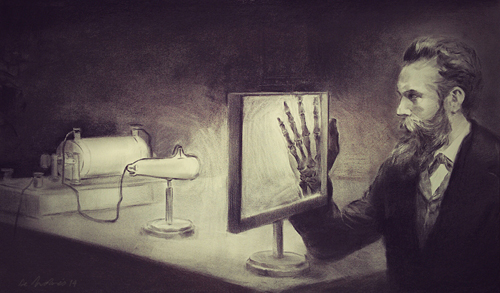
\includegraphics[width=64mm]{resources/15f.jpg} %Aquí se adjunta la foto como propiedad de la carpeta Resources
          };
      \end{tikzpicture}%
      
      \vfill
      \vfill
      \vfill
      \RaggedDown{Los rayos X se producen cuando se hace incidir un haz de electrones acelerados contra \'atomos de un material "blanco". Los electrones al chocar con los \'atomos del blanco, se frenan; perdiendo parte de su energ\'ia, que se termina irradiando en forma de calor y de ondas electromagn\'eticas: {\color{yellow}\textit{los rayos X}}}. 
    
    
    
    \end{frame}
    
    \section{Aplicaciones}
    \begin{frame}{Aplicaciones}
    \framesubtitle{Conociendo su uso cotidiano}
    \framsubsubtitle{\hspace{45mm}Medicina}
    \begin{multicols}{2}
    \begin{figure}
        \centering
        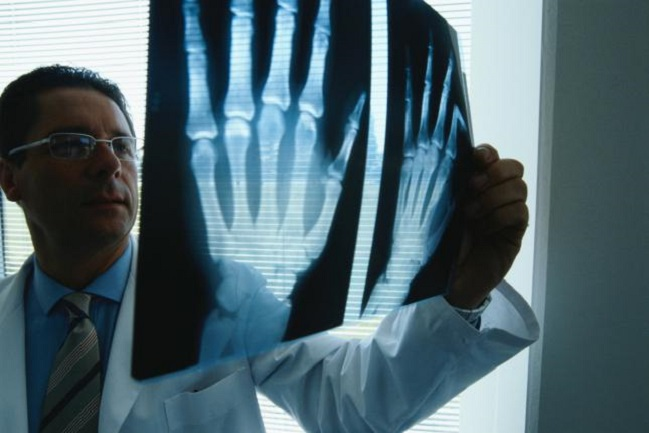
\includegraphics[width = 1.05 \linewidth]{resources/16f.jpg}
    \end{figure}
    
    \newpage
    \begin{figure}
        \centering
        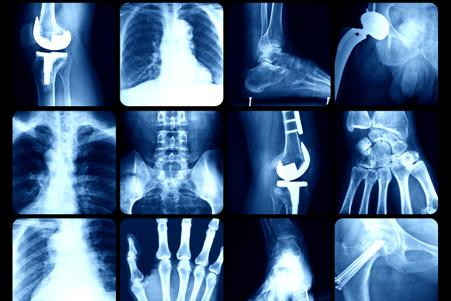
\includegraphics[width = 1.05 \linewidth]{resources/17f.jpg}
    \end{figure}
    
    \end{multicols}
    \Small{Figure: Son de las herramientas m\'as \'utiles para la detecci\'on de diversas enfermedades y condiciones y su posterior seguimiento.}
    \end{frame}
    
    \begin{frame}{Aplicaciones}
    \framesubsubtitle{\hspace{38mm}Espectroscop\'ia XPS}
    \begin{figure}
        \centering
        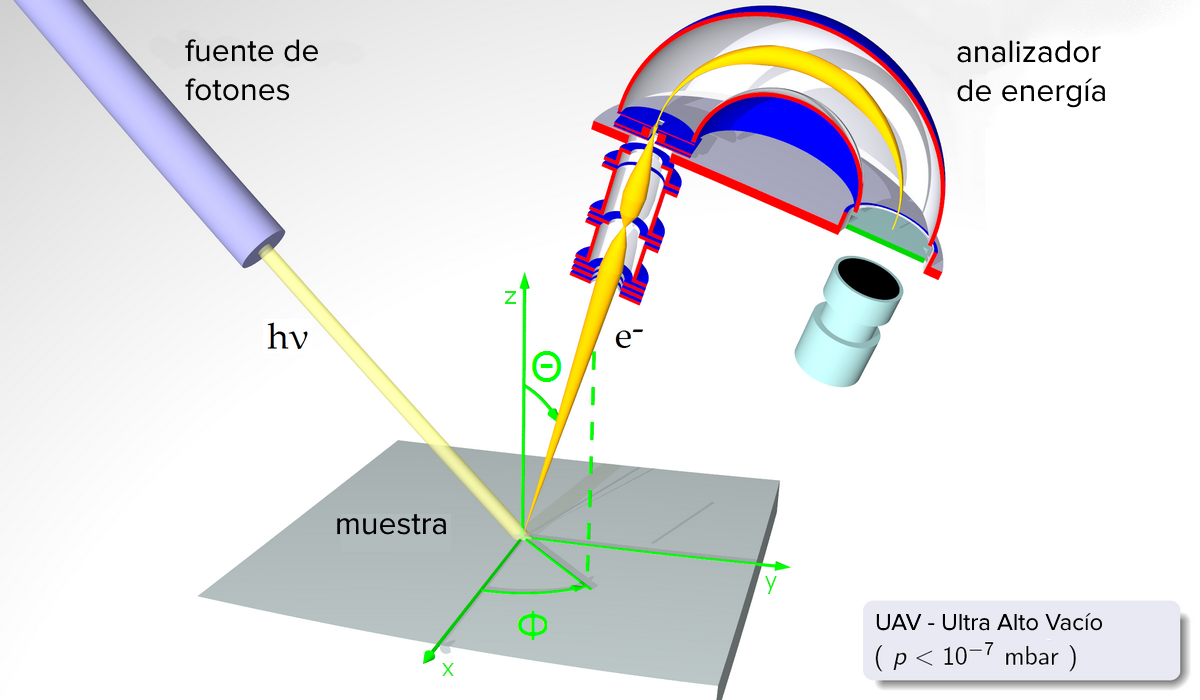
\includegraphics[width = 0.9 \linewidth]{resources/18f.png}
        \caption{Se usa mucho en investigaci\'on para el desarrollo de nuevos materiales y en controles de calidad de fabricaci\'on.}
        \label{fig:my_label}
    \end{figure}
    
    \end{frame}
    
    \begin{frame}{Aplicaciones}
    \framesubsubtitle{\hspace{45mm}Seguridad}
    \begin{figure}
        \centering
        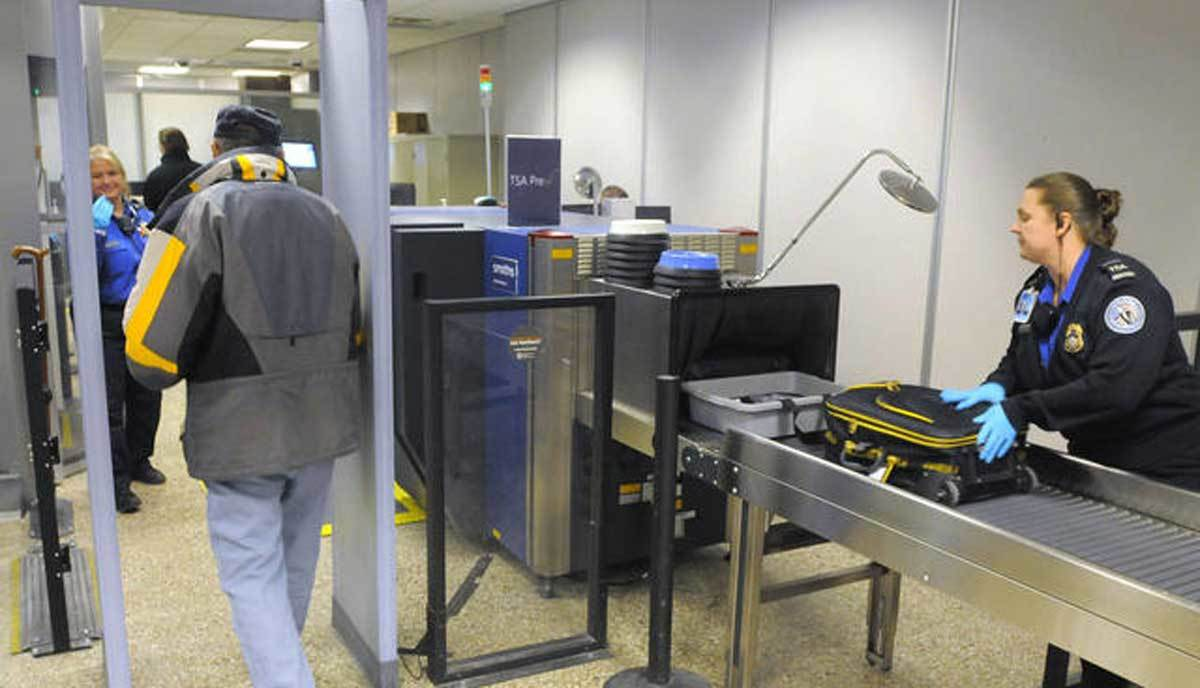
\includegraphics[width = 0.9 \linewidth]{resources/19f.jpg}
        \caption{Estos equipos pueden identificar armas y elementos met\'alicos que se encuentran ocultos en ropa, mochilas, maletas y dem\'as.}
        \label{fig:my_label}
    \end{figure}
    
    \end{frame}
    
    
    \section{Problemas}
    \begin{frame}{Ejercicio 1}
    \framesubtitle{Practicar es importante, chavos}
\begin{tikzpicture}[overlay,remember picture] %Comando para fotos que forman parte de la diapositiva
        \node[anchor=south east,xshift=-15pt,yshift=60pt] %Comando para mover la foto
          at (current page.south east) {
            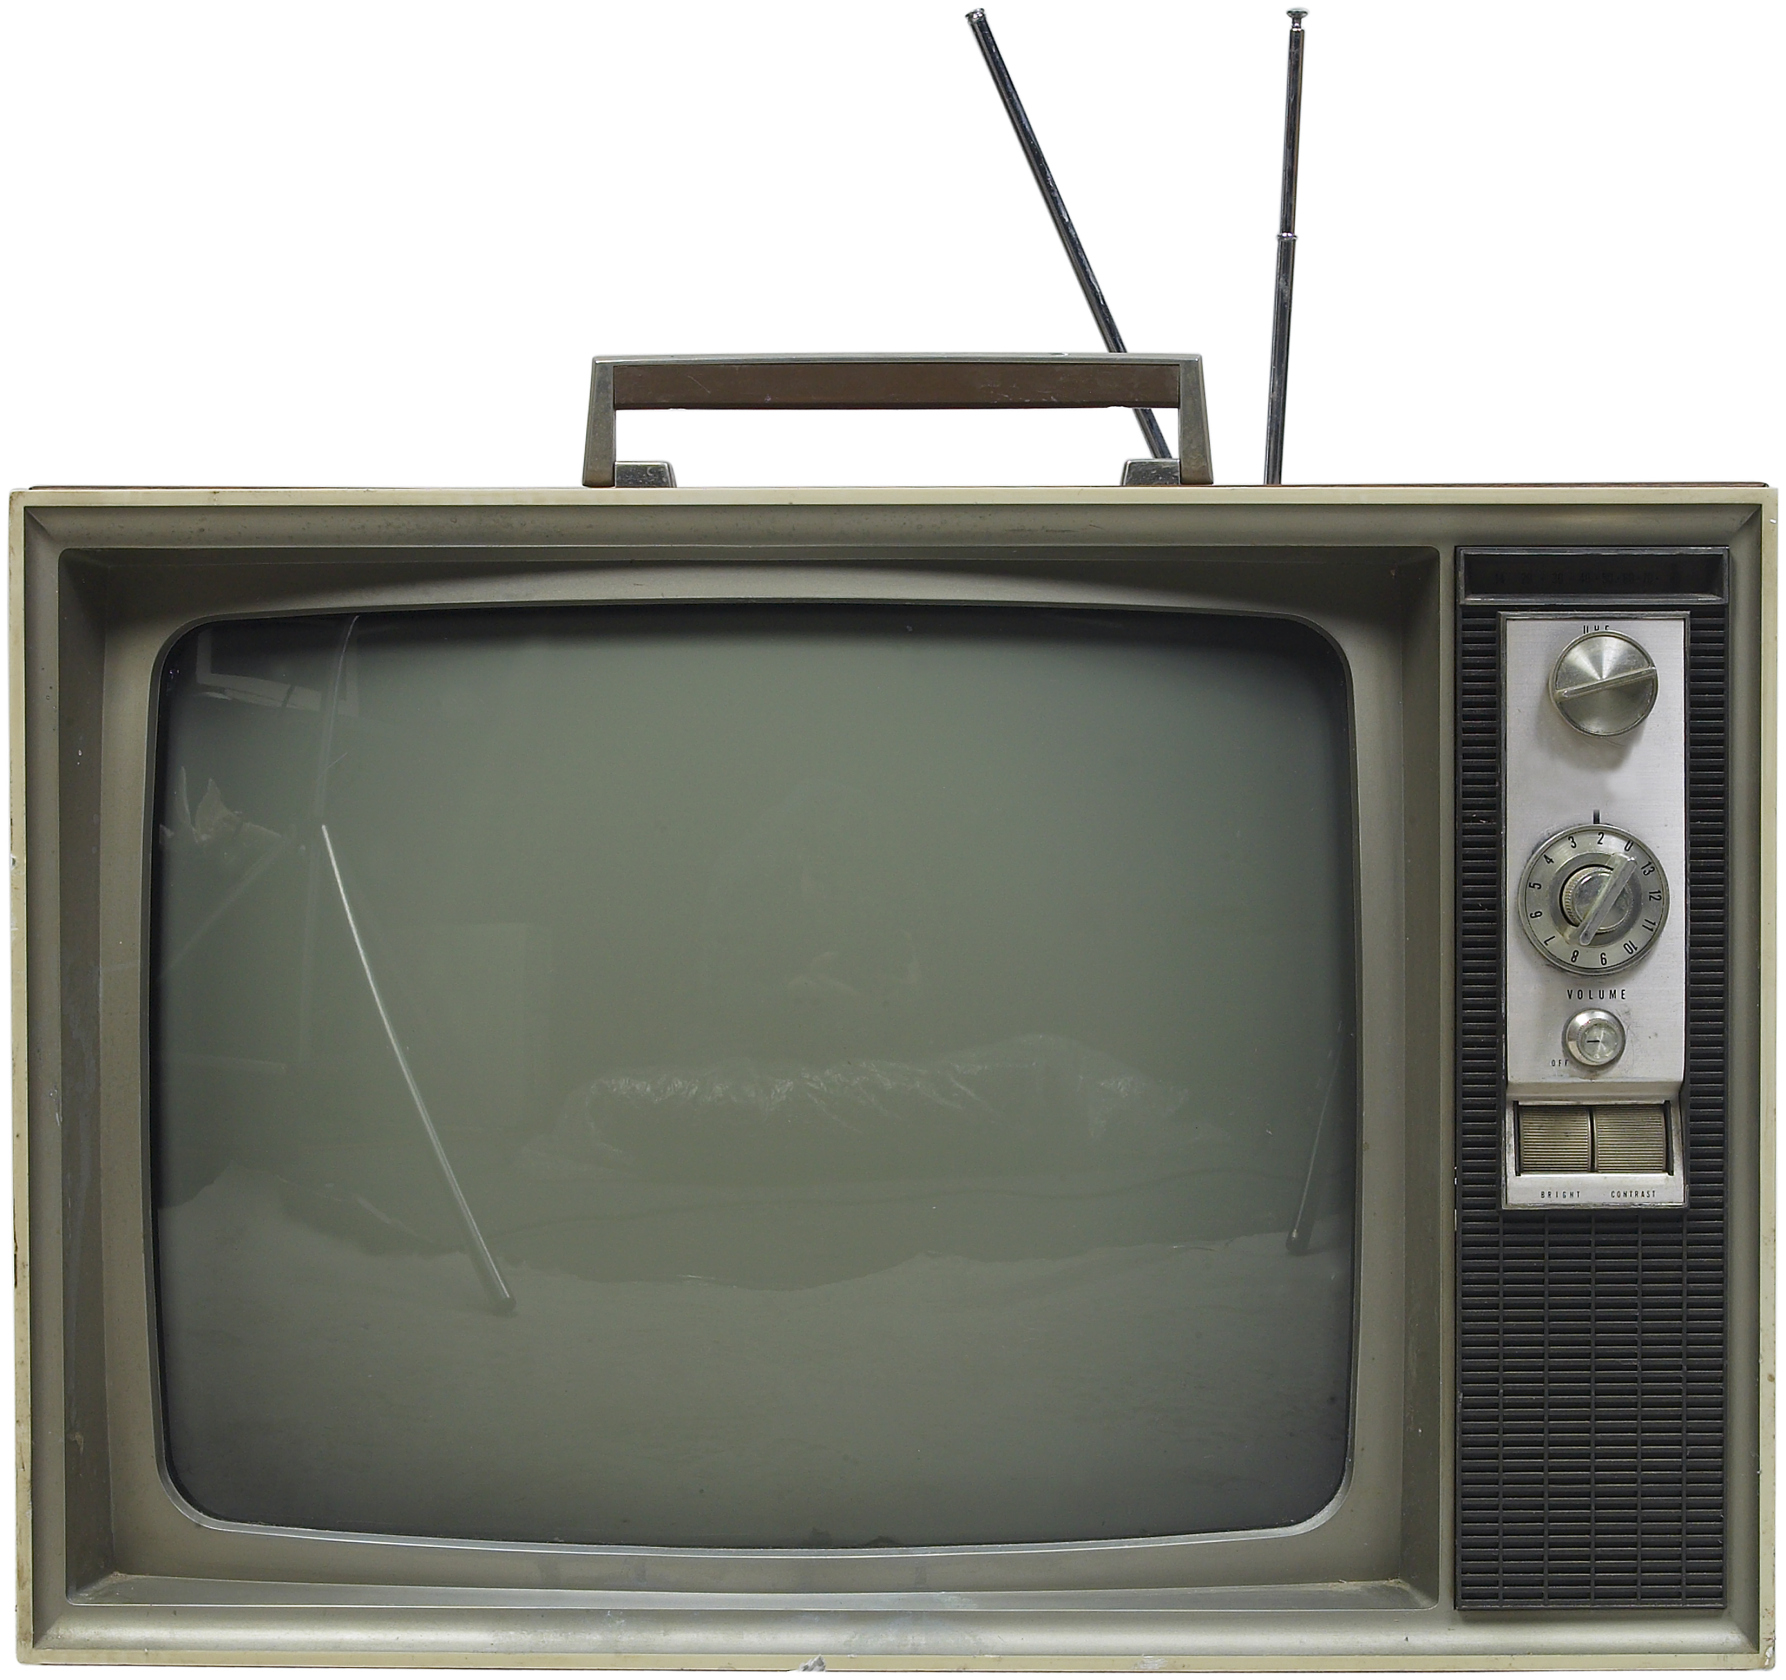
\includegraphics[width=30mm]{resources/25f.jpg} %Aquí se adjunta la foto como propiedad de la carpeta Resources
          };
      \end{tikzpicture}%
      
Un tubo de televisi\'on opera con un potencial de aceleraci\'on de $20 kV$. ¿Cuál es la m\'axima energ\'ia de los rayos X en la televisi\'on?


\bigskip
\framesubsubtitle{\textbf{Soluci\'on:}}


Los electrones en el tubo de la televisi\'on tienen 

una energ\'ia de $20 keV$, y si \'estos quedan en re-

poso despu\'es de un choque en el cual se emite 

un fot\'on de rayos X, la energía del fot\'on es de $20$

$keV$ y su longitud de onda es de

\begin{equation*}

    \lambda = \frac{c}{\nu} =\frac{hc}{h\nu} = \frac{12.4 keV \dot A}{20 keV} = 0.62 A
    
\end{equation*}

    
    \end{frame}


    \begin{frame}{Ejercicio 2}
        Los electrones son acelerados entre un filamento y una rejilla por una variable potencial $V$, atravesando un vapor de mercurio de por medio, como se muestra en el esquema. Un peque\~no potencial retardante $V_g \approx 0.5 V$ es mantenido entre la rejilla y la placa recolectora. 
        
        \begin{figure}
            \centering
            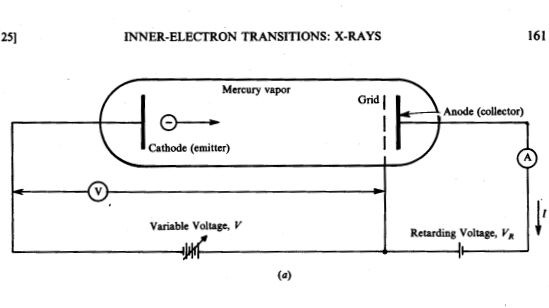
\includegraphics[width = 0.65 \linewidth]{resources/30f.png}
            \caption{Ejercicio 2: esquema del experimento}
            \label{fig:my_label}
        \end{figure}
        
    \end{frame}
    
    \begin{frame}{Ejercicio 2}    
        Cuando la intensidad $I$ es medida en la placa recolectora en funci\'on del voltaje de aceleraci\'on, las curvas de la gr\'afica son obtenidas. Determina la energ\'ia del primer estado de excitaci\'on del mercurio y la longitud de onda de la luz emitida en dicho estado.
    
        \begin{figure}
            \centering
            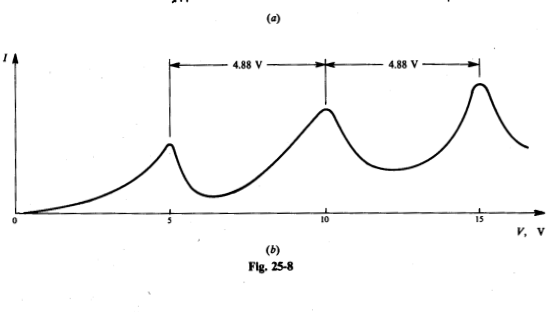
\includegraphics[width = 0.7 \linewidth]{resources/31f.png}
            \caption{Ejercicio 2: gr\'afica de $I$ vs $V$\\Intensidad de radiaci\'on vs voltaje}
            \label{fig:my_label}
        \end{figure}
        
    \end{frame}

    \section{Bibliograf\'ia} %Título que aparece en el índice
    \begin{frame}{Bibliograf\'ia} %Título que aparece en la diapositiva
      \framesubtitle{Referencias requeridas para la realizaci\'on del trabajo} %Subtítulo
      \begin{thebibliography}{9}
        \bibitem{knuth84}
            Homez L. Oswaldo I., “Fundamentos de f\'isica moderna: rayos X”, \url{https://slideplayer.es/slide/5518917/}
        \bibitem{lamport94}
            IAEA - Protecci\'on Radiol\'ogica de los Pacientes, “Rayos X”, \url{https://rpop.iaea.org/RPOP/RPoP/Content-es/InformationFor/Patients/patient-information-x-rays/index.htm}
        \bibitem{MG94}
           Pardell Xavier - Apuntes de electromedicina, “F\'isica de los Rayos X”, \url{https://www.pardell.es/fisica-de-los-rayos-x.html}

        \bibitem{tantau04}
            Pier D. Bruno, “F\'isica de los Rayos X”, \url{https://fr.slideshare.net/brunoipierdomenico/fisica-de-los-rayos-x-67651292}
      \end{thebibliography}
    \end{frame}
    
    \begin{frame}{Bibliograf\'ia} %Título que aparece en la diapositiva
      \begin{thebibliography}{9}
        \bibitem{knuth84}
            Gatreau R., Savin W., “Theory and problems of modern physics”, \url{https://vinaire.files.wordpress.com/2017/04/schaum-modern-physics.pdf}
       
      \end{thebibliography}
    \end{frame}

  \end{darkframes}


\end{document}


